\begin{center}

\includegraphics[width=0.3\textwidth]{content/3/chapter4/images/44.png}\\
Cippi已经为比赛做好了准备
\end{center}

C++20对属性进行了改进,并添加了新的属性,如[[nodiscard("reason")]]、[[likely]]、[[unlikely]]和[[no\_unique\_address]]。并且,[[nodiscard("reason")]]可以用来显式地表达接口的意图。


\begin{tcolorbox}[breakable,enhanced jigsaw,colback=blue!5!white,colframe=blue!75!black,title={属性}]

属性允许开发者对源代码进行约束,或者为编译器提供优化可能性。可以为类型、变量、函数、名称和代码块使用属性。使用多个属性时,可以依次应用(func1),或者在一个属性中一起应用,用逗号(func2)分隔:

\hspace*{\fill} \\ %插入空行
\noindent
\textbf{使用属性}
\begin{lstlisting}[style=styleCXX]
[[attribute1]] [[attribute2]] [[attribute3]]
int func1();

[[attribute1, attribute2, attribute3]]
int func2();
\end{lstlisting}

属性可以是实现定义的语言扩展或标准属性,下面是C++11至C++17的已有属性列表。

\begin{itemize}
\item 
{}[[noreturn]] (C++11): 表示函数不返回

\item 
{}[[carries\_dependency]] (C++11): 表示\href{https://en.cppreference.com/w/cpp/atomic/memory_order#Release-Consume_ordering}{release-consume内存序}依赖链中的依赖项

\item 
{}[[deprecated]] (C++14):表示不再使用的名称

\item 
{}[[fallthrough]] (C++17): 表示有意跳过一个分支

\item 
{}[[maybe\_unused]] (C++17): 抑制编译器对未使用名称的警告
\end{itemize}
\end{tcolorbox}


\subsubsubsection{4.8.1\hspace{0.2cm} [[nodiscard("reason")]]}

C++17毫无理由地引入了新的属性[[nodiscard]]。C++20增加了向属性中添加信息的可能性。

\hspace*{\fill} \\ %插入空行
\noindent
\textbf{丢弃对象和错误码}
\begin{lstlisting}[style=styleCXX]
// withoutNodiscard.cpp

#include <utility>

struct MyType {

	MyType(int, bool) {}

};

template <typename T, typename ... Args>
T* create(Args&& ... args) {
	return new T(std::forward<Args>(args)...);
}

enum class ErrorCode {
	Okay,
	Warning,
	Critical,
	Fatal
};

ErrorCode errorProneFunction() { return ErrorCode::Fatal; }

int main() {

	int* val = create<int>(5);
	delete val;
	
	create<int>(5);
	
	errorProneFunction();
	
	MyType(5, true);

}
\end{lstlisting}

因为转发和参数包,工厂函数create(第11行)可以调用构造函数,并返回一个在堆上分配的对象。

这段代码有很多问题。首先,第30行存在内存泄漏,堆上创建的int永远不会删除。其次,没有检查函数errorProneFunction(第32行)的错误代码。最后,构造函数调用MyType(5, true)(第34行)创建一个临时对象,创建后立即销毁,这至少是一种资源浪费。现在,让[[nodiscard]]发挥作用吧。

[[nodiscard]]可以在函数声明、枚举声明或类声明中使用。若丢弃了声明为[[nodiscard]]的函数的返回值,编译器应该发出警告。通过复制枚举或声明为[[nodiscard]]的类返回的函数也是如此。若仍然想忽略返回值,可以将其强制转换为void。

下面的例子中,使用了C++17的属性[[nodiscard]]。

\begin{lstlisting}[style=styleCXX]
// nodiscard.cpp

#include <utility>

struct MyType {

	MyType(int, bool) {}

};

template <typename T, typename ... Args>
[[nodiscard]]
T* create(Args&& ... args){
	return new T(std::forward<Args>(args)...);
}

enum class [[nodiscard]] ErrorCode {
	Okay,
	Warning,
	Critical,
	Fatal
};

ErrorCode errorProneFunction() { return ErrorCode::Fatal; }

int main() {

	int* val = create<int>(5);
	delete val;
	
	create<int>(5);
	
	errorProneFunction();
	
	MyType(5, true);

}
\end{lstlisting}

工厂函数create(第13行)和enum ErrorCode(第17行)声明为[[nodiscard]]。因此,第31行和第33行中在使用时,触发了警告。

\begin{center}
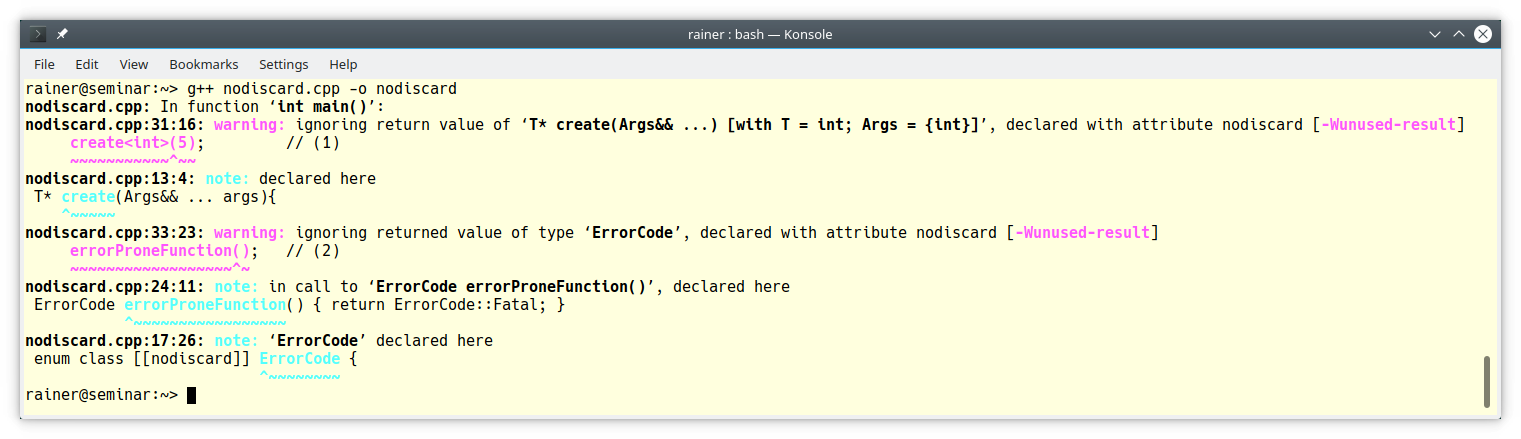
\includegraphics[width=0.8\textwidth]{content/3/chapter4/images/45.png}\\
C++17编译器会报错
\end{center}

这样就好多了,但这段代码还有一些问题。[[nodiscard]]不能用于构造函数等不返回值的函数,所以临时的MyType(5, true)(第35行)仍会创建,并且没有警告。第二,错误消息太一般。作为函数的使用者,我想知道为什么丢弃结果这一行为是有问题的。

这两个问题都可以用C++20解决。构造函数可以声明为[[nodiscard]],警告可以包含其他信息。

\hspace*{\fill} \\ %插入空行
\noindent
\textbf{C++20中使用[[nodiscard]]属性}
\begin{lstlisting}[style=styleCXX]
// nodiscardString.cpp

#include <utility>

struct MyType {

	[[nodiscard("Implicit destroying of temporary MyInt.")]] MyType(int, bool) {}
	
};

template <typename T, typename ... Args>
[[nodiscard("You have a memory leak.")]]
T* create(Args&& ... args){
	return new T(std::forward<Args>(args)...);
}

enum class [[nodiscard("Don't ignore the error code.")]] ErrorCode {
	Okay,
	Warning,
	Critical,
	Fatal
};
 
ErrorCode errorProneFunction() { return ErrorCode::Fatal; }

int main() {

	int* val = create<int>(5);
	delete val;
	
	create<int>(5);
	
	errorProneFunction();
	
	MyType(5, true);

}
\end{lstlisting}

现在,将输出特定的消息。下面是Microsoft编译器的输出。

\begin{center}
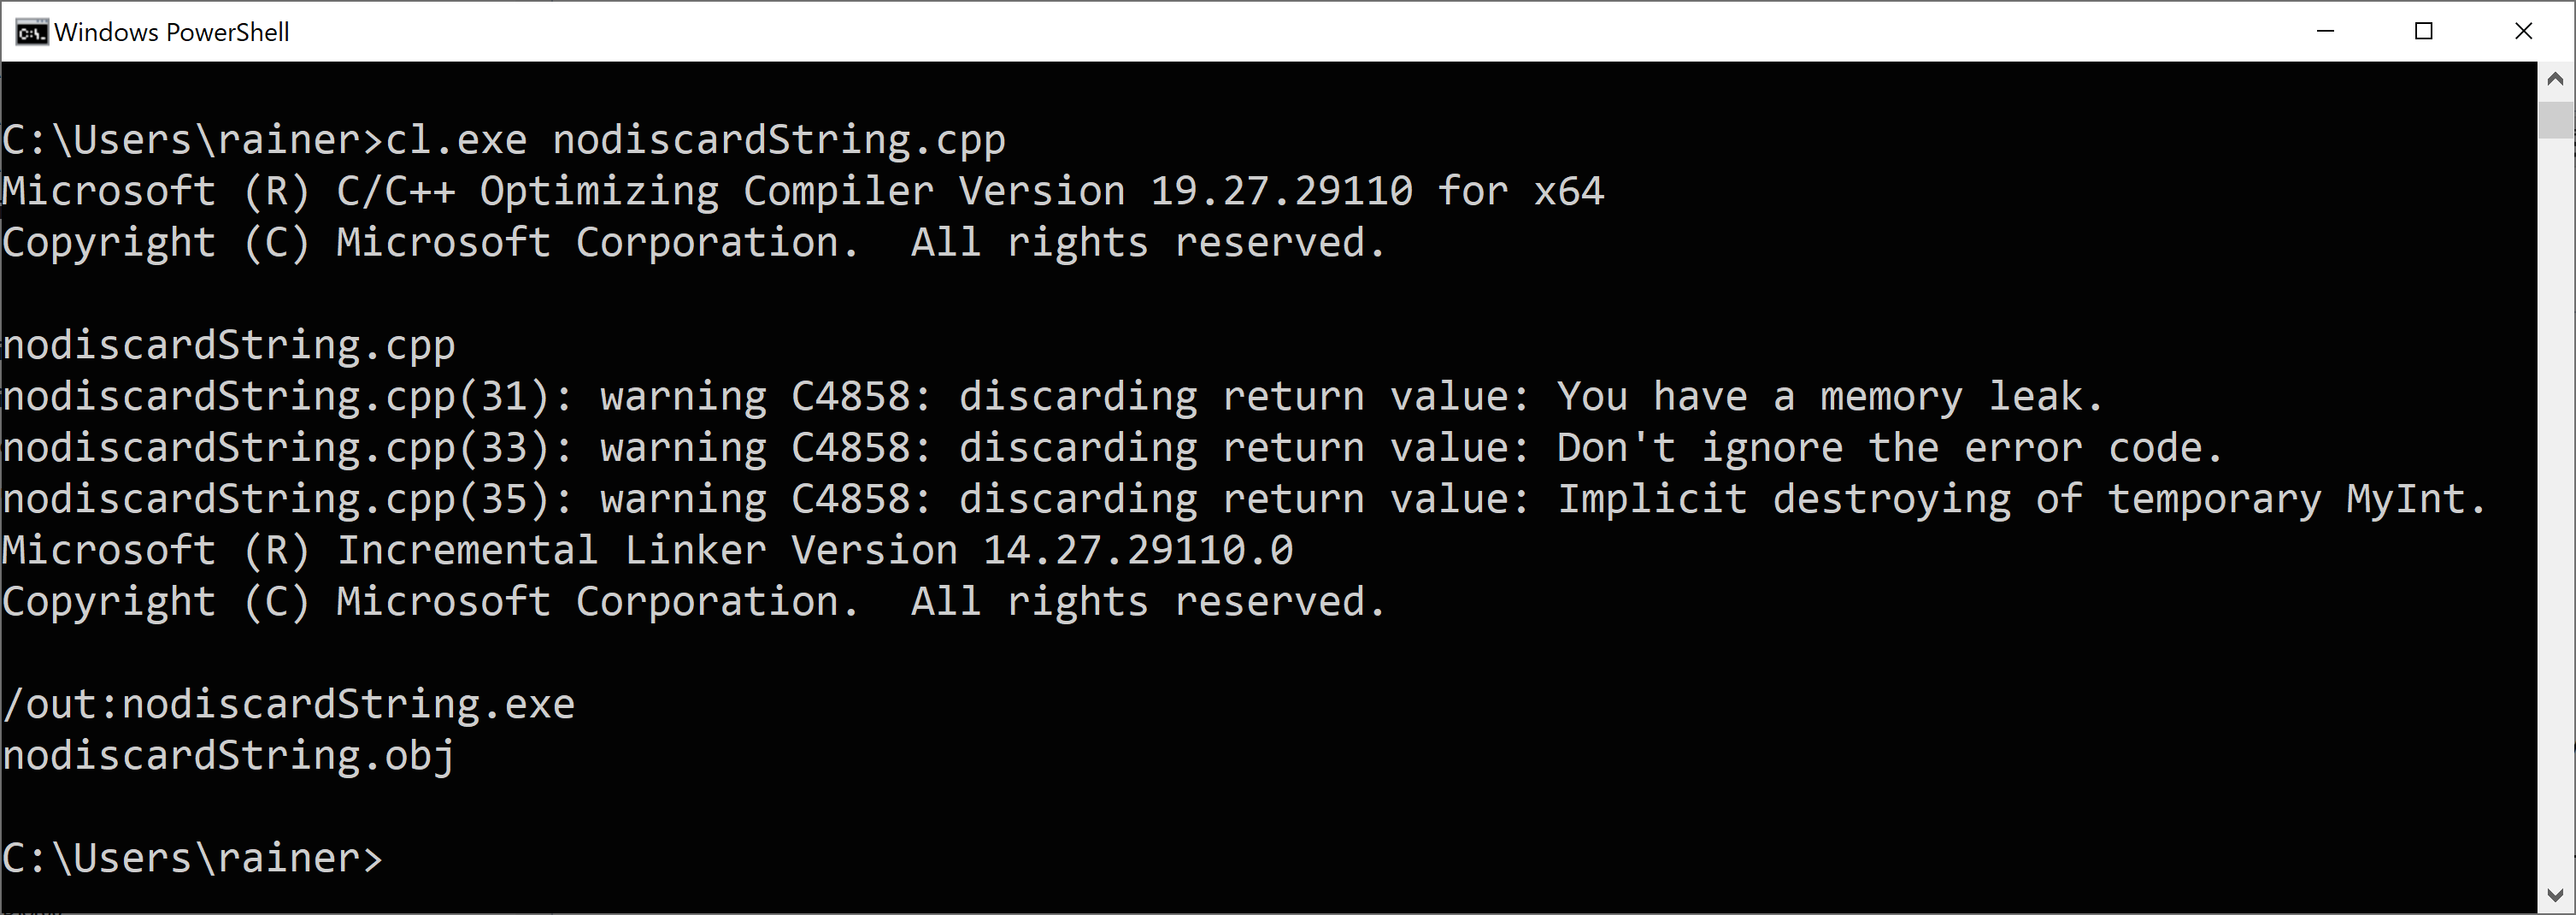
\includegraphics[width=1.0\textwidth]{content/3/chapter4/images/46.png}\\
C++20编译器会对丢弃对象和错误代码的行为报错
\end{center}

\begin{tcolorbox}[breakable,enhanced jigsaw,colback=red!5!white,colframe=red!75!black,title={std::async的问题}]
	
C++中的许多函数都可以使用[[nodiscard]]属性,并从中获益,其中就包括std::async。当不使用std::asnyc的返回值时,想要std::async异步使用隐式地转变为同步使用。应该在单独的线程中运行的内容,但却以阻塞的方式使用。更多关于std::async的反直觉行为,请参阅我的帖子\href{https://www.modernescpp.com/index.php/the-special-futures}{“the-special-futures”}。

\hspace*{\fill} \\ %插入空行
研究\href{https://en.cppreference.com/w/cpp/language/attributes/nodiscard}{cppreference.com/nodiscard}上的[[nodiscard]]语法时,我注意到\href{https://en.cppreference.com/w/cpp/thread/async}{std::async}的声明在C++20中发生了变化:

\hspace*{\fill} \\ %插入空行
\noindent
\textbf{std::async在C++20中使用属性[[nodiscard]]}
\begin{lstlisting}[style=styleCXX]
template<class Function, class... Args>
[[nodiscard]]
std::future<std::invoke_result_t<std::decay_t<Function>,
								 std::decay_t<Args>...>>
	async( Function&& f, Args&&... args );
\end{lstlisting}

std::async的返回类型在C++20中声明为[[nodiscard]]。
	
\end{tcolorbox}

接下来的两个属性[[likely]]和[[unlikely]]是关于优化的。

\subsubsubsection{4.8.2\hspace{0.2cm}[[likely]]和[[unlikely]]}

[[likely]]和[[unlikely]]属性的提案\href{http://www.open-std.org/jtc1/sc22/wg21/docs/papers/2018/p0479r5.html}{P0479R5}据我所知是最短的。为了说明动机,提案中添加了有趣的注释。“可能属性的使用旨在允许实现针对以下情况进行优化:语句或标签上,包含该属性的执行路径比不包含该属性的执行路径的可能性都要大。使用unlikely属性是为了允许实现针对以下情况进行优化:语句或标签上,包含该属性的执行路径比不包含该属性的执行路径更不可能。当执行路径包含到该标签的跳转时,包含该标签。不过,过度使用这些属性都可能导致性能的下降。”总而言之,这两个属性都会向优化器提供与预期执行路径相关的提示。

\hspace*{\fill} \\ %插入空行
\noindent
\textbf{[[likely]]:给优化器一个提示}
\begin{lstlisting}[style=styleCXX]
for(size_t i=0; i < v.size(); ++i){
	if (v[i] < 0) [[likely]] sum -= sqrt(-v[i]);
	else sum += sqrt(v[i]);
}
\end{lstlisting}

优化的过程继续使用新的属性[[no\_unique\_address]],这个优化处理的是空间上的,而不是执行时间上的。

\subsubsubsection{4.8.3\hspace{0.2cm} [[no\_unique\_address]]}

[[no\_unique\_address]]表示类中的成员变量不需要有内存地址。若成员为空类型,编译器可以将其优化为不占用内存。

下面的程序演示了新属性的用法。

\hspace*{\fill} \\ %插入空行
\noindent
\textbf{使用[[no\_unique\_address]]属性}
\begin{lstlisting}[style=styleCXX]
// uniqueAddress.cpp

#include <iostream>

struct Empty {};

struct NoUniqueAddress {
	int d{};
	[[no_unique_address]] Empty e{};
};

struct UniqueAddress {
	int d{};
	Empty e{};
};

int main() {

	std::cout << '\n';
	
	std::cout << std::boolalpha;
	
	std::cout << "sizeof(int) == sizeof(NoUniqueAddress): "
			  << (sizeof(int) == sizeof(NoUniqueAddress)) << '\n';
	
	std::cout << "sizeof(int) == sizeof(UniqueAddress): "
			  << (sizeof(int) == sizeof(UniqueAddress)) << '\n';
	
	std::cout << '\n';
	
	NoUniqueAddress NoUnique;
	
	std::cout << "&NoUnique.d: " << &NoUnique.d << '\n';
	std::cout << "&NoUnique.e: " << &NoUnique.e << '\n';
	
	std::cout << '\n';
	
	UniqueAddress unique;
	
	std::cout << "&unique.d: " << &unique.d << '\n';
	std::cout << "&unique.e: " << &unique.e << '\n';
	
	std::cout << '\n';

}
\end{lstlisting}

NoUniqueAddress类的大小等于int(第7行),但UniqueAddress类的大小不等于int(第12行)。UniqueAddress的成员d和e(第40行和41行)有不同的地址,但UniqueAddress类的成员没有(第33行和34行)。

\begin{tcblisting}{commandshell={}}
sizeof(int) == sizeof(NoUniqueAddress): true
sizeof(int) == sizeof(UniqueAddress): false

&NoUnique.d: 0x7fff44f8fd0c
&NoUnique.e: 0x7fff44f8fd0c

&unique.d: 0x7fff44f8fd04
&unique.e: 0x7fff44f8fd08
\end{tcblisting}

\begin{tcolorbox}[breakable,enhanced jigsaw,colback=mygreen!5!white,colframe=mygreen!75!black,title={总结}]
C++20添加了一些新的属性:
\begin{itemize}
\item 
{}[[nodiscard("reason")]]可以在上下文中检查函数的返回值是否忽略。

\item 
{}[[likely]]和[[unlikely]]允许开发者给编译器一个提示,哪个代码路径更有可能执行到。

\item 
使用[[no\_unique\_address]]属性,类中不同的成员变量可以拥有相同的地址。
\end{itemize}
\end{tcolorbox}

\newpage
















